\chapter{Solução Proposta: \textit{Clean Pool Robot}}
\section{Visão Global}
O \textit{Clean Pool Robot} é um robô de aspiração de fundos de piscinas. O
mecanismo do mesmo será composto por dois métodos para que o fundo da piscina
possa ser aspirado: o primeiro baseia-se na escovação do chão e o segundo a
sucção das impurezas desprendidas do piso da piscina.
\par
O primeiro método tem foco nas escovas que estão situadas na parte inferior
do robô. As escovas realizam movimentos giratórios fazendo com que suas cerdas
entrem em contato com o chão retirando  impurezas, como por exemplo: algas e
grãos de terra.
\par
Após a escovação, é realizado outro método, a sucção das impurezas desprendidas
do piso da piscina  além de outras impurezas que estiverem próximas à área de
atuação do robô, por exemplo: pequenos ramos e folhas. Por meio de uma bomba, a
água é sugada por uma abertura situada na parte inferior e passa por um saco onde
as partículas de maiores dimensões ficam depositadas. Depois de passar pelo saco,
a água passa por um filtro removível. As impurezas menores ficam retidas no filtro.
Por meio de um sistema de expulsão de água, esta sairá a uma velocidade muito superior
à velocidade de entrada no início do processo, ajudando também na movimentação do robô.
\par
Com o término da limpeza na piscina, haverá a necessidade dos filtros serem limpos
para retirada das impurezas colhidas na aspiração da água. Assim, após cada utilização
o usuário deverá limpar os filtros internos do \textit{Clean Pool Robot}.
\par
O produto desenvolvido será responsável apenas pela retirada da sujeira decantada
no fundo da piscina, ou seja, o \textit{Clean Pool Robot} não limpará as paredes
ou superfície da piscina. Além disso, as piscinas ideais para a operação do Robot
são as retangulares, sem inclinações e azulejadas. É ideal também que o robô seja
lançado na piscina no meio da largura maior, evitando que o fio fique totalmente
esticado quando o robô estiver na quina oposta do lançamento.
\par
Como diferencial, o \textit{Clean Pool Robot} será um produto nacional com custo
mais acessível e que possui percurso não aleatório.
\par
O \textit{Clean Pool Robot} pode ser dividido em duas grandes partes, uma compondo a
estrutura (apelidada de corpo) e o outro a parte lógica (apelidada de mente) do
robô. Cada uma dessas será explicada posteriormente.

\section{Percurso do Robô}
O esquemático abaixo mostra uma ideia inicial de como o robô percorrerá a piscina
a ser limpada.
\par
\begin{figure}[h]
    \centering
    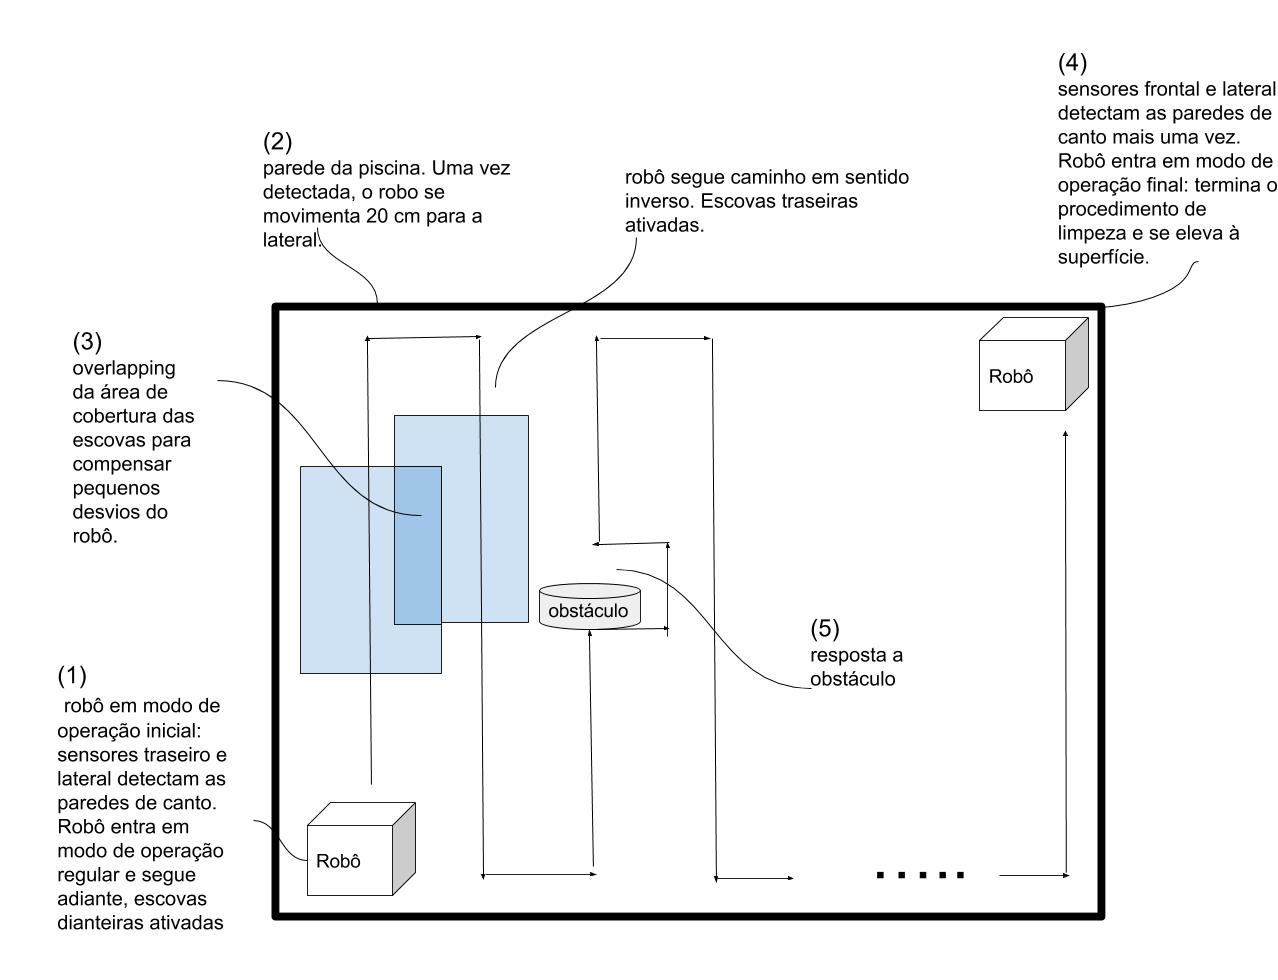
\includegraphics[width=\textwidth]{figures/schema-way-robot.jpg}
    \caption{Demonstrativo do percurso de limpeza do robô.}
    \label{fig:schema-way-robot}
  \end{figure}
\par
O robô limpador foi projetado para ser capaz de percorrer toda a área da superfície
inferior de piscinas retangulares e sem inclinação. A varredura é feita de forma
totalmente autônoma pelo sistema, com a \textit{Raspberry pi} como unidade central de
controle de todos elementos periféricos: sensores de distância, servo motores,
sensores de pressão, etc. É necessário o usuário apenas posicionar o limpador em
uma das bordas da piscina e recolhê-lo quando o processo de limpeza estiver completo.
\par
Com o intuito de simplificar o sistema, optou-se por permitir ao robô mover-se apenas
em duas direções, horizontal e vertical, em ambos os sentidos. Desta forma,
baseando-se em projetos similares como o descrito na patente \textit{POOL CLEANER
DIRECTIONAL CONTROL METHOD AND APPARATUS} (2001, patent No:US 6,299,699 B1), o
padrão ideal de varredura consiste em uma sequência de travessias longitudinais
paralelas, partindo de uma borda da piscina à outra, como pode ser visto na figura
acima.
\par
O limpador inicia o processo de varredura assim que os sensores de distância,
localizados em cada uma das laterais do robô, detectam que ele se encontra em
uma das quinas da piscina (1).  O limpador segue em linha reta em direção à
próxima parede, com os motores das escovas ativados para fazer a limpeza do chão.
Uma vez próximo à parede, limpador então desloca-se para a direita cerca de 20
centímetros e segue o percurso em linha reta, em sentido contrário (2). O deslocamento
de 20 centímetros é tal que haja uma sobreposição das áreas varridas pelas escovas
em ambos os sentidos percorridos (3), de forma a compensar qualquer desvio de
rota não detectado pelo giroscópio. O limpador retorna à parede inicial, desloca-se
outros 20 centímetros para a direita  e segue mais uma vez em sentido oposto. Este
procedimento se repete até que o robô chegue à parede direita da piscina (4). Na
eventualidade de o robô se encontrar, no meio do percurso,  com um obstáculo grande
o bastante para ser detectado pelos sensores de distância, o limpador deverá desviar
do obstáculo e seguir sua rota original (5).

\section{Modos de Operação}
A movimentação do robô limpador é definida por quatro modos de operação distintos,
referentes às quatro etapas de funcionamento: inicial, operação regular,
resposta a obstáculo e final.
\par
Na etapa inicial, o limpador deve ser capaz de submergir ao fundo da piscina e
posicionar-se em um dos quatro vértices. Uma vez posicionado ele inicia o modo
de operação regular e realiza o percurso de limpeza  explicado anteriormente.
Terminado o percurso, o robô deve ser capaz de “emergir” à superfície para ser
coletado pelo usuário. Caso o limpador se depare com um obstáculo de grande porte
em seu percurso, ele deve ser capaz de circundar o obstáculo e retornar ao modo de
operação regular.

\subsection{Modo de Operação Regular}
O fluxograma a seguir define com mais detalhes as lógicas de funcionamento
do robô limpador para o modo de operação regular, levando em conta todos os
componentes eletrônicos envolvidos.
\par
\begin{figure}[h]
  \centering
  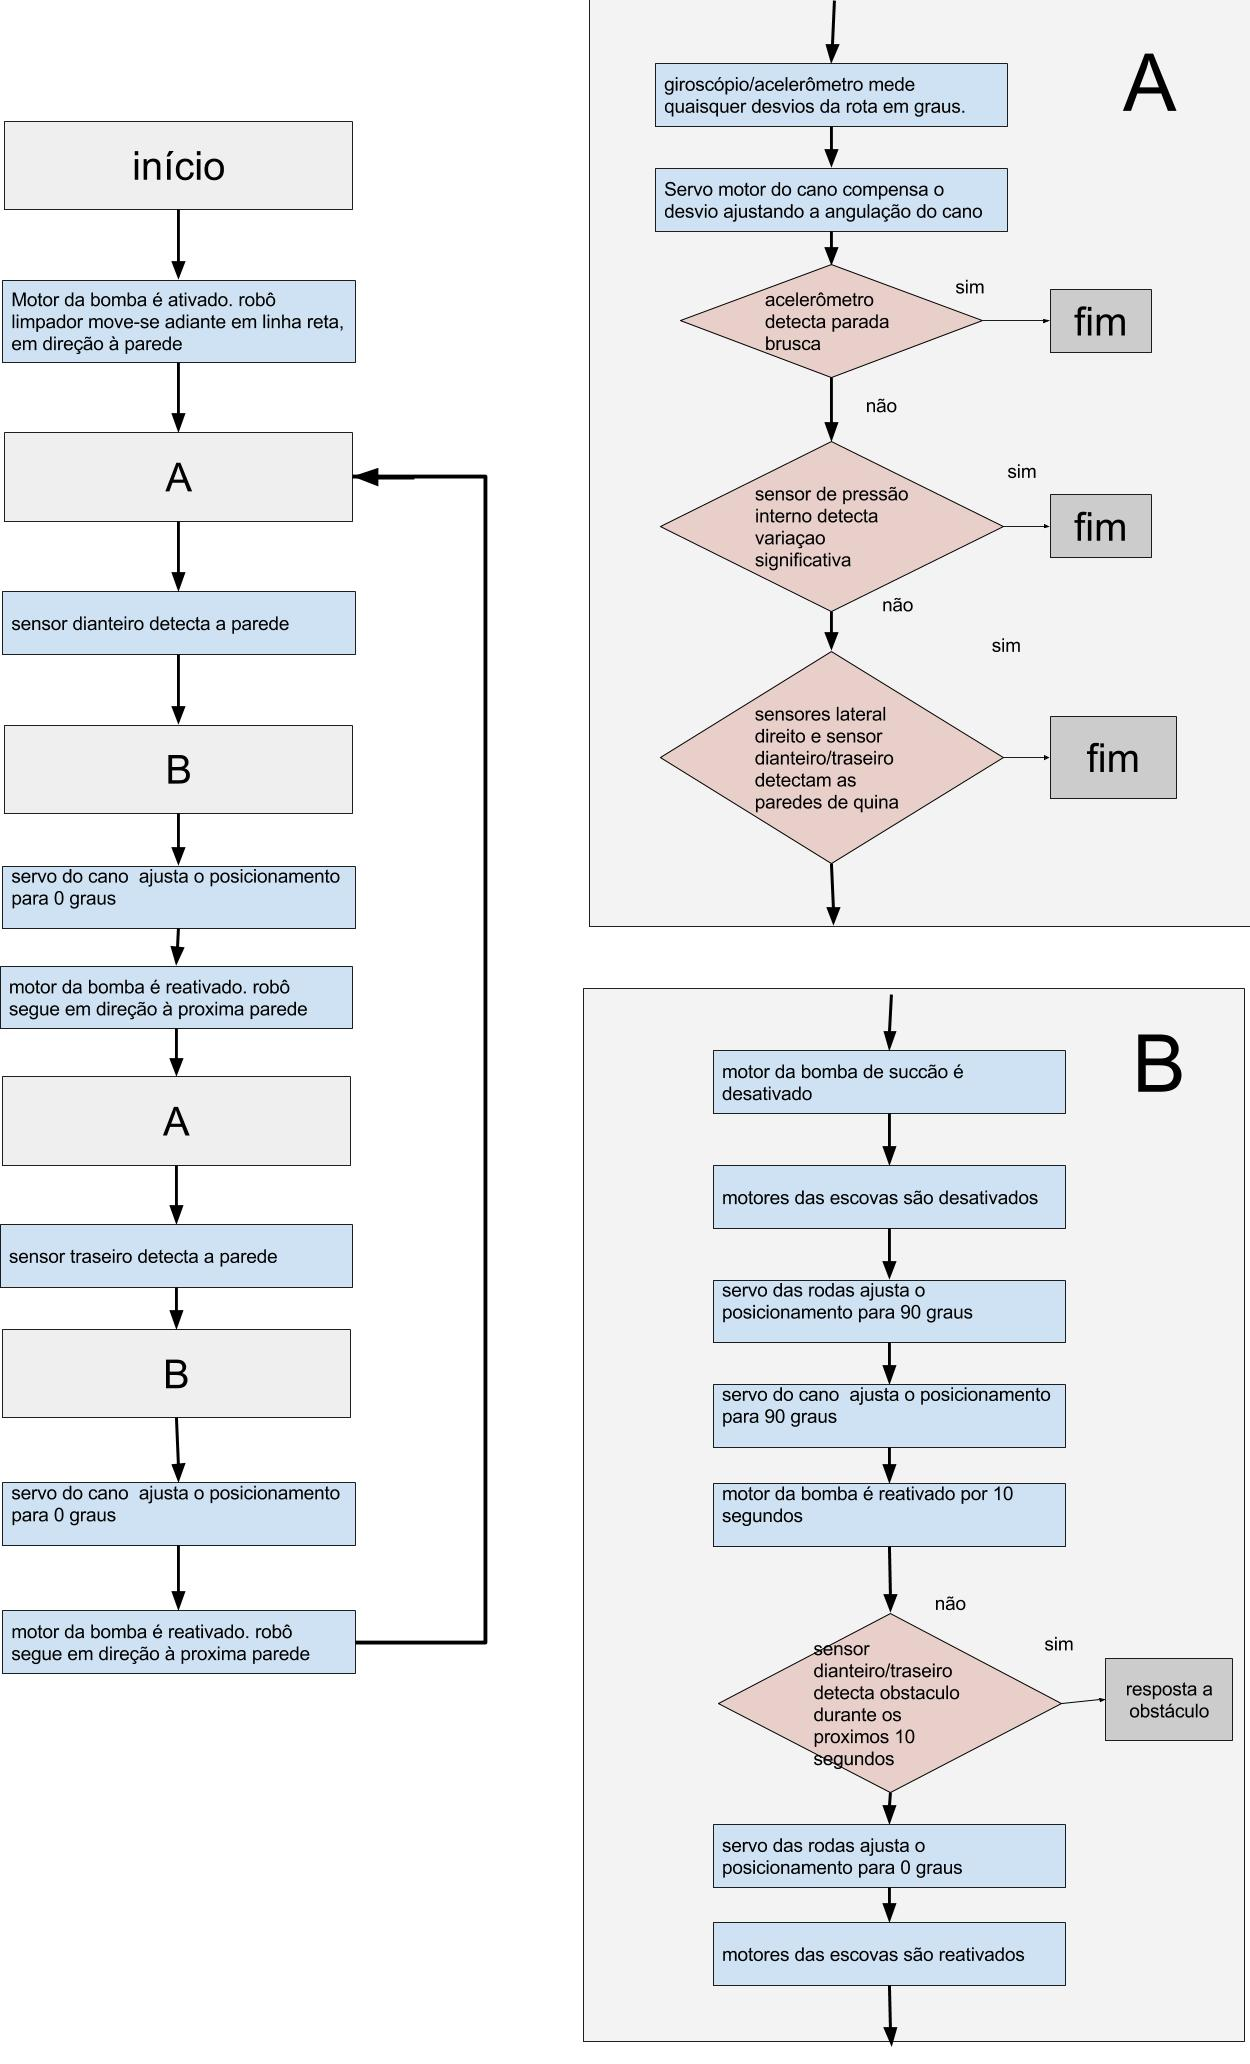
\includegraphics[width=0.9\textwidth]{figures/flow-regular-robot.jpg}
  \caption{Modo de Operação Regular do \textit{Clean Pool Robot}}
  \label{fig:flow-regular-robot}
\end{figure}
\FloatBarrier

\subsection{Resposta a Obstáculos}
Foram definidos três casos de obstáculo que o robô poderá encontrar em seu percurso.

\begin{description}
\item[Caso 1:] \textit{Obstáculo pequeno capaz de ser sugado pela bomba e obstruir os
filtros do limpador}. Neste caso, o sensor de pressão interna detecta qualquer
variação de pressão na caixa do filtro.  A operação de limpeza é então abortada
e o robô para e se “eleva à superfície” (modo de operação final).
\item[Caso 2:] \textit{Obstáculo grande não detectado pelos sensores, resultando em
colisão direta com obstáculo}. Neste caso, o acelerômetro detecta parada brusca
do robô. A operação de limpeza é  também abortada e o robô para e se” eleva à
superfície” (modo de operação final).
\item[Caso 3:] \textit{Obstáculo grande e detectável pelos sensores de distância}. O
robô não é capaz de imediatamente discernir a parede da piscina com o obstáculo
e segue, a princípio, com seu procedimento como se o obstáculo fosse de fato parede.
\end{description}
\par
O fluxograma a seguir detalha em alto nível de abstração as etapas que o sistema
de controle devem seguir para circundar o obstáculo neste caso
\par
\begin{figure}[h]
  \centering
  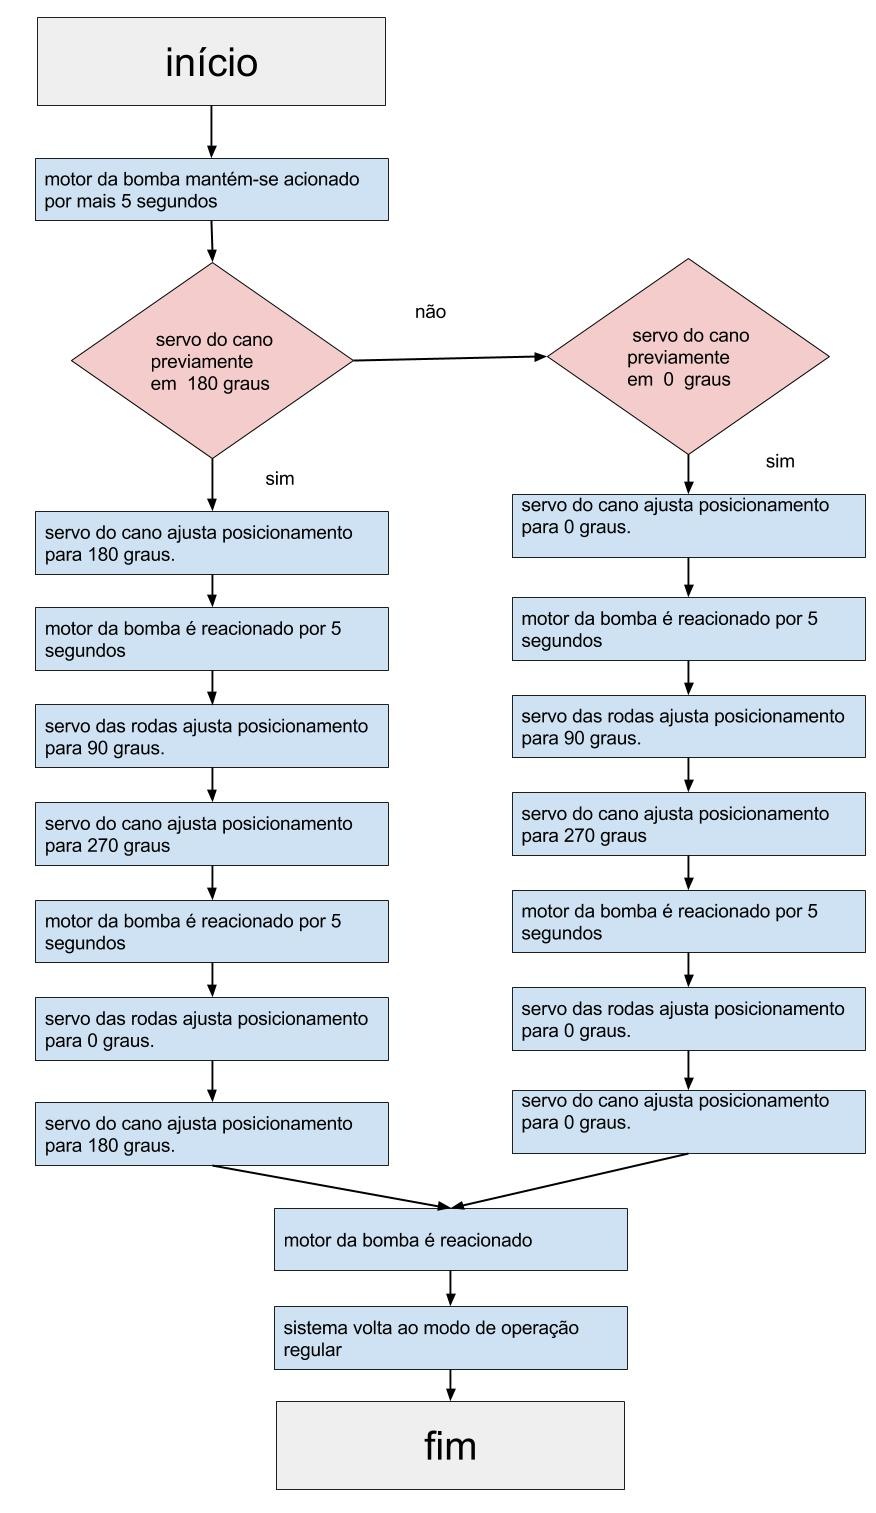
\includegraphics[width=0.9\textwidth]{figures/flow-robot-obstacle.jpg}
  \caption{Modo de Operação Resposta a Obstáculos do \textit{Clean Pool Robot}}
  \label{fig:flow-obstacle-robot}
\end{figure}
\FloatBarrier

\subsection{Modo de Operação Inicial e Final}
Antes de começar a varredura da piscina, o robô deve primeiro posicionar-se
perfeitamente em um dos 4 cantos da piscina. O fluxograma a seguir detalha
as etapas do processo a partir do momento em que o limpador chega ao fundo
da piscina.
\par
\begin{figure}[h]
  \centering
  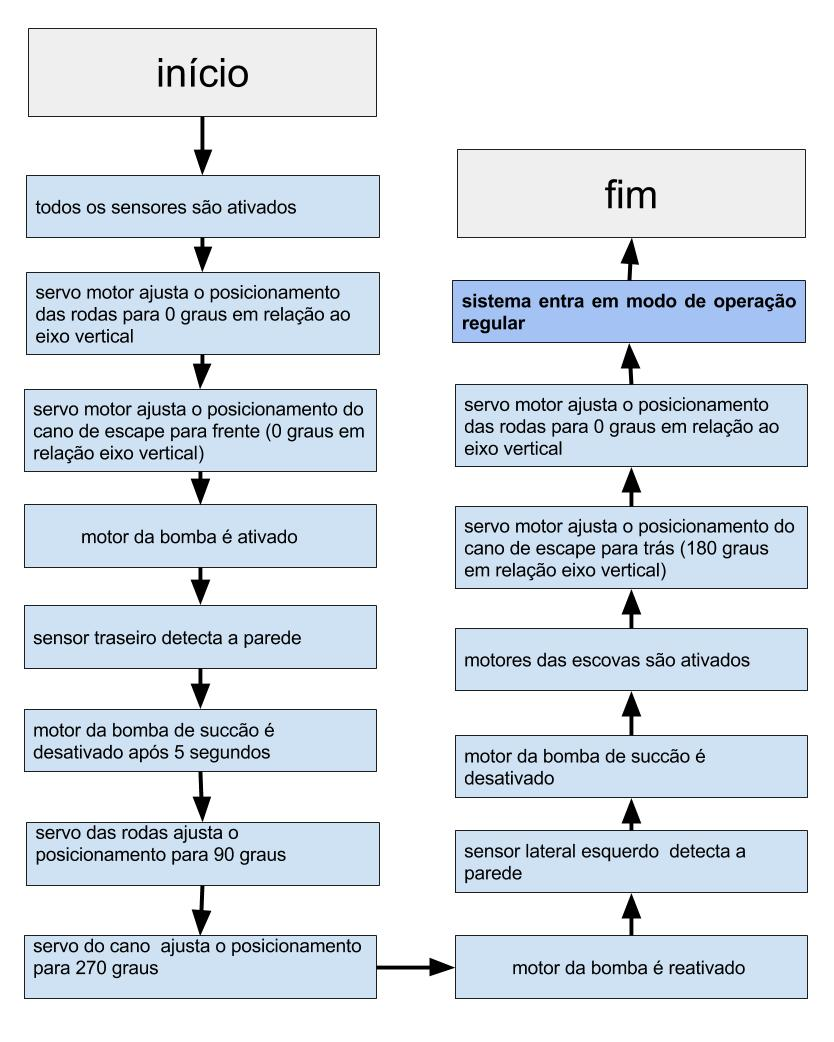
\includegraphics[width=0.9\textwidth]{figures/flow-initial-robot.jpg}
  \caption{Modo de Operação Inicial e Final do \textit{Clean Pool Robot}}
  \label{fig:flow-initial-robot}
\end{figure}
\FloatBarrier

\section{O Corpo do Robô (Aeroespacial, Automotiva e Energia)}
A figura abaixo mostra a primeira modelagem do\textit{Clean Pool Robot}. O modelo
apresenta uma bomba de sucção (1), uma caixa com os filtros para as impurezas
(2), dois motores para a rotação das escovas (3), uma saída superior da água
filtrada (4), quatro rodas próprias para rolagem em ambientes aquáticos (5),
dois enrolamentos com escovas para soltura da sujeira do piso da piscina (6),
duas entradas para sucção da água e impurezas do fundo da piscina (7), uma
entrada da fonte de alimentação externa (8) e uma caixa com os circuitos
eletrônicos do robô (9). Abaixo da figura estão detalhados as especificações
de cada componente utilizado no Robô.
\par
\begin{figure}[h]
  \centering
  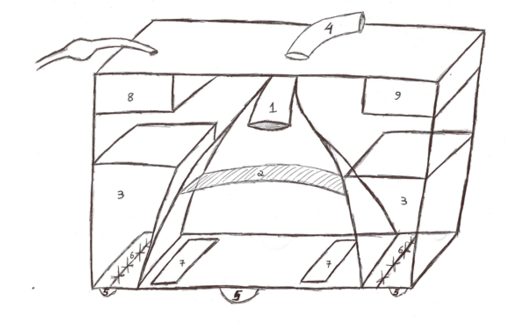
\includegraphics[width=0.9\textwidth]{figures/croqui.png}
  \caption{ Croqui inicial do \textit{Clean Pool Robot}}
  \label{fig:initial_croqui}
\end{figure}
\FloatBarrier
\par
Por motivo de resistência ao movimento o formato do robô foi modificado para
melhor aproveitamento das forças aerodinâmica envolvidas, as alterações no
desenho inicial foram feitas com a intenção de diminuir a força de arrasto, a
estrutura conta agora com cantos e arestas arredondadas conforme a Figura.
\par
\begin{figure}[h]
  \centering
  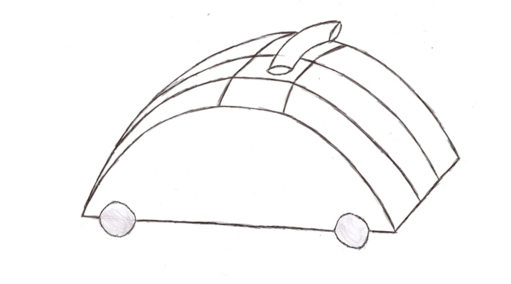
\includegraphics[width=0.9\textwidth]{figures/better-croqui.png}
  \caption{ Croqui melhorado do \textit{Clean Pool Robot}}
  \label{fig:better-croqui}
\end{figure}
\FloatBarrier
\par
\begin{description}
\item[Bomba:] O processo de aspiração da piscina feito pelo robô será uma das
principais tarefas executadas pela bomba de sucção, bem como também o processo
de movimentação do robô embaixo d’água. Para isso, é importante que a bomba
seja resumidamente forte o suficiente para sugar e gerar movimentação por meio
do fluxo de saída da bomba. A sucção será conectada diretamente ao reservatório
onde acontecerá a filtragem da água. Com isso, é esperado que a vazão diminua
entorno de 30 a 40\% da sua vazão nominal de saída. É importante ressaltar que
as únicas funções da bomba neste projeto são apenas filtrar e movimentar por empuxo.
\par
A análise do dimensionamento adequado para a bomba será feito a partir de sua vazão
nominal. Para isto, tem-se por especificações primárias bombas que ofereçam vazões
altas e que trabalhem em uma profundidade máxima de 3 metros. 
\par
Após o cálculo de sua velocidade de saída utilizando a sua vazão e área de jato,
serão calculados o empuxo desenvolvido e sua respectiva pressão de saída. É importante
salientar que a pressão de saída deverá ser sempre positiva e superior a pressão
hidrostática a qual está submetido o bocal de propulsão.
\par
Ao longo de alguns estudos, observou-se que para o problema dado os modelos de bombas
que melhor se enquadram são as moto bombas, uma vez que as mesmas possuem baixo peso e
altas velocidades de saída, bem como altas vazões.
\par
O modelo parcialmente proposto será uma bomba do tipo Bilge , na qual tem as seguintes
características:
  \begin{itemize}
  \item Peso: aproximadamente 3 kg;
  \item Modelo: 500 GPH - com Tensão de trabalho 12 V DC - Amperagem de 1.9;
  \item Formato: Cilíndrico alterável;
  \item Área de operação entorno de até 3,7 metros.
  \end{itemize}
\par
\begin{figure}[h]
  \centering
  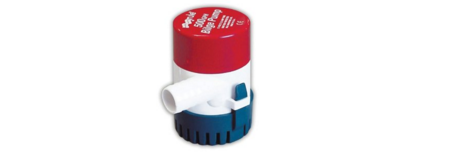
\includegraphics[width=0.9\textwidth]{figures/waterbomb.png}
  \caption{Bomba proposta}
  \label{fig:waterbomb}
\end{figure}
\FloatBarrier
\par
\textit{Dimensionamento do Teste:} Diante de todo processo de dimensionamento
e a propulsão do robô abaixo d’água, foi pensado em um teste para analisar se
há coerência nos cálculos realizados. Sendo assim, o teste irá ser realizado
com um uma estrutura móvel e uma bomba de aquário. É esperado, com isso, validar
os cálculos realizados no que tange a movimentação da estrutura. Para isso,
foram explicados por meio dos métodos de cálculos descritos a seguir. Segundo
ISE(2000), quando um veículo submersível se movimenta com velocidade constante,
a propulsão gerada pelos propulsores se iguala à força de arrasto produzida. A
força de arrasto será obtida a partir da soma da força de arrasto devido a 
movimentação do veículo mais a força de arrasto devido o cabo de alimentação.
\begin{displaymath}
  Fp = Fa = Fv + Fc = \frac{1}{2}\rho V^{2}_{v}Cd_{v} + \frac{1}{2}\rho V^{2}_{c}Cd_{c}
\end{displaymath}
Onde $Fp$ e $Fa$ referem-se à força de propulsora e força de arrasto total
respectivamente, $Fv$ e $Fc$ são as forças de arrasto devido ao veiculo e ao cabo de
alimentação, $\rho$ é a densidade do fluido, $V_{v}$ e $V_{c}$ velocidades do
veículo e do cabo e por fim, $Cd_{v}$ e $Cd_{c}$ representam os coeficientes
de arrasto.
\par
A potência necessária para a bomba pode ser obtida em função da força propulsiva
e da velocidade do veiculo.
\begin{displaymath}
  P = Fp\frac{d}{t}
\end{displaymath}
Onde $d$ é a distancia percorrida, $t$ o tempo e $P$ a potência desejada.
\par
Os coeficientes de arrasto são medidos experimentalmente, para fluidos como
ar podem ser encontrados tabelados em função da velocidade do veiculo em relação
à velocidade do som nas condições do ambiente em questão (número de \textit{Mach}), uma
vez que este pode sofrer alterações devido a temperatura envolvida, meio de
propagação etc. Quando o veículo estudado se movimento em fluido líquido como a
água por exemplo, o coeficiente de arrasto deve ser medido em função do número
de Reynolds, (Eng et al., 2008) que por sua vez é calculado pela equação abaixo.
\begin{displaymath}
  Re = \frac{VD}{\upsilon}
\end{displaymath}
Onde $V$ equivale a velocidade do veículo, $D$ o diâmetro e $\upsilon$ a viscosidade
cinemática do fluido.
\par
\begin{figure}[h]
  \centering
  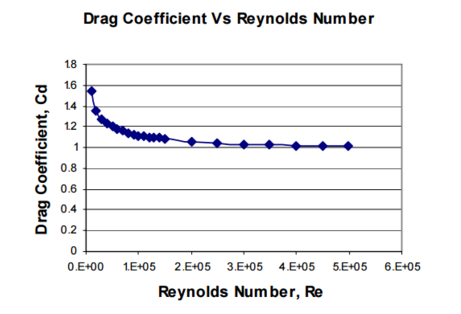
\includegraphics[width=0.9\textwidth]{figures/graphic-reynolds.png}
  \caption{Coeficiente de arrasto em função do numero de Reynolds}
  \label{fig:graphic-reynolds}
\end{figure}
\FloatBarrier
\par
Inicialmente a bomba utilizada será uma bomba de aquário, o que servirá de
parâmetro para a determinação da bomba correta. Para isso, serão realizados
testes com essa bomba para comprovação dos cálculos descritos acima.

\item[Sistema Filtrador:] O sistema de filtragem irá garantir que a piscina
estará limpa após o uso do \textit{Clean Pool Robot}. O filtro será fundamental,
pois ele será responsável pela remoção das partículas de sujeira que ficam decantado
no fundo da piscina. Primeiro a água será sugada para dentro do aparelho que passará por
um depósito onde será feita a filtragem. Em seguida, a água filtrada retorna para
piscina. Será realizado um sistema de dupla filtragem com dois tipos de elementos
filtrantes, um de malha, secundário, para evitar que folhas e objetos de maior
tamanho entrem no filtro principal que será responsável por filtrar o particulado
e detritos da água.
\begin{itemize}
  \item Filtros: Usar-se-á uma malha de alumínio para a realização de uma
  pré-filtragem, a qual impedirá que folhas, plásticos, cabelos, e outros
  materiais maiores entupam o filtro principal responsável por retirar impurezas
  menores da água. Essa malha é o que chamaremos de filtro secundário. O filtro
  principal será um elemento filtrante na forma cilíndrica comumente utilizado
  na filtragem de caixas d’águas. As imagens dos filtros a serem utilizados e as
  especificações técnicas do elemento filtrante principal constam a seguir.
  \item Malha de Alumínio: A malha de alumínio é uma grade localizada na entrada
  da caixa filtradora, no duto de acesso na base do robô, conforme imagem abaixo.
  \par
  \begin{figure}[h]
    \centering
    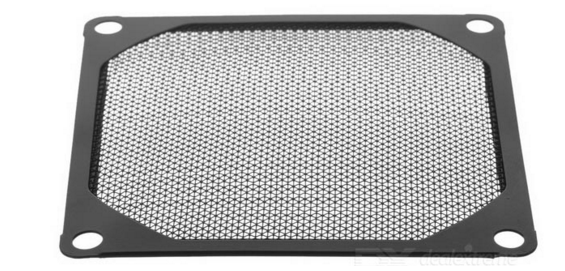
\includegraphics[width=0.9\textwidth]{figures/mesh-aluminium.png}
    \caption{Modelo de malha de alumínio utilizada como filtro secundário.}
    \label{fig:mesh-aluminium}
  \end{figure}
  \FloatBarrier
\end{itemize}

\item[Motor:] Serão utilizados dois motores elétricos para rotacionar as escovas.
a transmissão do torque para as escovas será por engrenagens, como ilustrado na
Figura.
\par
\begin{figure}[h]
  \centering
  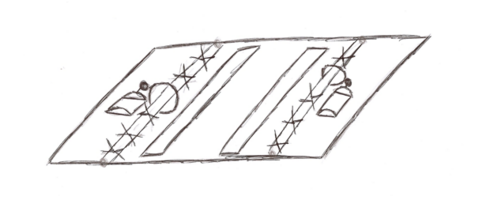
\includegraphics[width=0.9\textwidth]{figures/eletric-motor.png}
  \caption{Atuação do motor elétrico.}
  \label{fig:eletric-motor}
\end{figure}
\FloatBarrier

\item[Saída Supeior de Água:] A água que é ejetada do sistema de filtragem é
devolvida para a piscina já filtrada, auxiliando assim a limpeza geral de todo
o volume em que o robô esta submerso. A água filtrada é direcionada para uma
saída que se localiza na parte superior do produto. O duto de saída possui quatro
aberturas imediatamente opostas que servem para direcionar o jato d’água,
funcionando como o sistema de propulsão do produto. Quando uma das quatro aberturas
estiverem sendo utilizadas para direcionar o jato, as outras três permanecem
fechadas sendo utilizadas somente quando for necessário para a movimentação para a
direção desejada.

\item[Rodas:] O aparelho contará com dois tipos de rodas, a primeira em formato
de esfera que será apenas para apoio. Foram utilizadas quatro rodas desse modelo.
A segunda roda será para direcionar o aparelho no seu movimento, e será localizada
no centro do robô, conforme imagem abaixo. A roda central será responsável pela
alteração de direção do robo, sendo que apenas efetuará giros de  90º.
\par
\begin{figure}[h]
  \centering
  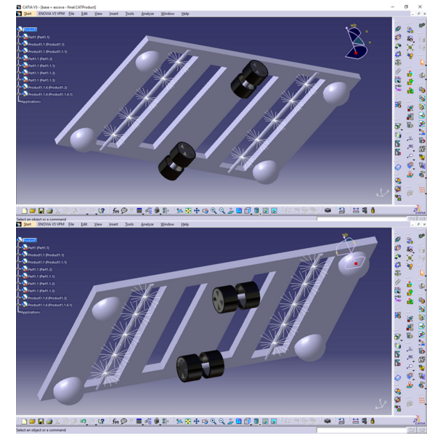
\includegraphics[width=0.9\textwidth]{figures/wheels.png}
  \caption{Localização das rodas e rotação das rodas centrais.}
  \label{fig:wheels}
\end{figure}
\FloatBarrier

\item[Escovas:] Imaginou-se utilizar escovas de formato cilíndrico, afim de que
à medida que as rodas do robô se movem, as escovas também possam acompanhar o
movimento sem maiores problemas. As cerdas da escova devem possuir elevada
resistência à tração, resistência à fadiga, baixo coeficiente de atrito e boa
resistência térmica. Dessa forma como material para as cerdas sugere-se o
Nylon (Santos, 2010).
\par
\begin{figure}[h]
  \centering
  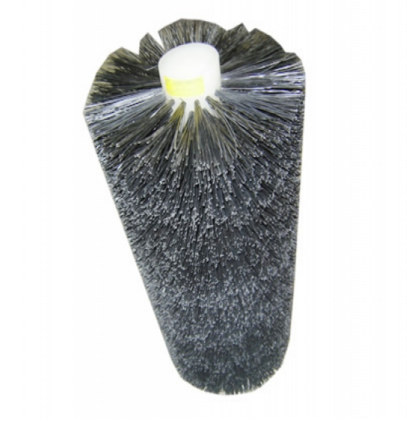
\includegraphics[width=0.4\textwidth]{figures/brush.png}
  \caption{Modelo de escova sugerido para a limpeza da piscina.}
  \label{fig:wheels}
\end{figure}
\FloatBarrier
A localização das escovas está ilustrada na figura \ref{fig:wheels}, feita no software
\textsf{CAD Catia V5 R19}. Serão utilizadas duas escovas movidas por motores elétricos,
que farão a limpeza do chão.
\par
\begin{figure}[h]
  \centering
  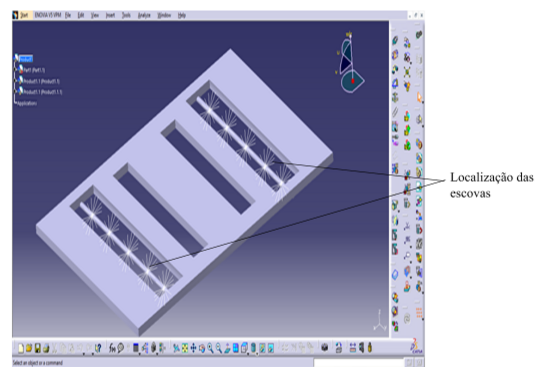
\includegraphics[width=0.8\textwidth]{figures/brush-local.png}
  \caption{Localização das escovas no robô.}
  \label{fig:brush-local}
\end{figure}
\FloatBarrier
\par
A movimentação das escovas será realizada por meio de engrenagens, como ilustrados
na Figura abaixo. O motor elétrico fornecerá um torque e o sistema de
engrenagem transmitirá para o eixo, fazendo com que as escovas rotacionem.
\par
\begin{figure}[h]
  \centering
  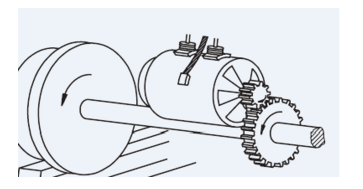
\includegraphics[width=0.8\textwidth]{figures/brush-system.png}
  \caption{Sistema para movimentação das escovas.}
  \label{fig:brush-system}
\end{figure}
\FloatBarrier

\item[Entrada Inferior d'água:] As entradas ficará localizada logo após as
escovas, como pode ser observado na figura \ref{fig:better-croqui}.

\item[Fonte de Alimentação Externa:] O \textit{Clean Pool Robot} é alimentado por
uma fonte de energia que fica fora da água, através de um cabo de força. O Robô
será alimentado pela tomada perto da piscina, em tensão de 220V (padrão Brasília).
O cabo de alimentação terá um extensão que garante o deslocamento do robô por todas
as extremidades da piscina durante a sua limpeza. Para o dimensionamento do
comprimento do cabo foi calculado uma distância da tomada até a borda da piscina,
somado ao maior comprimento possível para deslocamento do robô. Assim o comprimento
do fio é dado por:
\begin{displaymath}
  L= d + D
\end{displaymath}
Onde o $L$ é o comprimento total do cabo de energia do robô, $d$ é a distância da
tomada até a borda da piscina e $D$ é a distância a borda até o fundo da
extremidade oposta a ela. Assim o cabo terá $L = 16,6 \approx 17m$. Considerando que
a entrada do cabo na piscina se fará no ponto $P_ {ent}$, na metade da piscina,
conforme a figura abaixo.
\par
\begin{figure}[h]
  \centering
  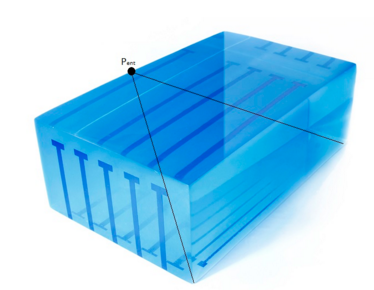
\includegraphics[width=0.8\textwidth]{figures/cable-desloc.png}
  \caption{Deslocamento do cabo dentro da piscina.}
  \label{fig:cable-desloc}
\end{figure}
\FloatBarrier
\par
O cabo de energia possuirá uma boia presa ao logo da sua extensão para evitar
enrolamento do cabo e possível ruptura do mesmo. O fio possuirá um revestimento
de PVC impermeável e uma bitola estimada de 3,5 mm, para um potência consumida
total de 350W.

\item[Vedação:] É o processo que impede a passagem de líquidos, gases e
sólidos particulados de um meio para outro. O material do vedador deve ser
compatível com o produto para que não ocorra reações químicas causando vazamento
e contaminação do produto.
\par
\begin{figure}[h]
  \centering
  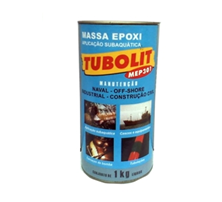
\includegraphics[width=0.5\textwidth]{figures/haha.png}
  \caption{Massa Epoxi para vedação.}
  \label{fig:haha}
\end{figure}
\FloatBarrier
\par
A massa Epoxi Tubolit Mep 301 funciona como proteção anti-corrosiva, proteção
contra impactos, solda a frio, isolante elétrico, reparos em geral de furos,
emendas e enchimentos, tanto dentro quanto fora d’água. Para aplicação
subaquática: Manutenção Nava, Off-shore, Industrial, Construção Civil. Para
revestimento e reparo em aço, concreto e outros materiais. Estruturas parcial
ou totalmente submersas, oleodutos, hidroelétricas, plataforma de petróleo,
estacas de concreto, tanques, reservatórios e caixas d'água.
\end{description}

\section{A Mente Do Robô (Eletrônica e Software)}
\par
\begin{figure}[h]
  \centering
  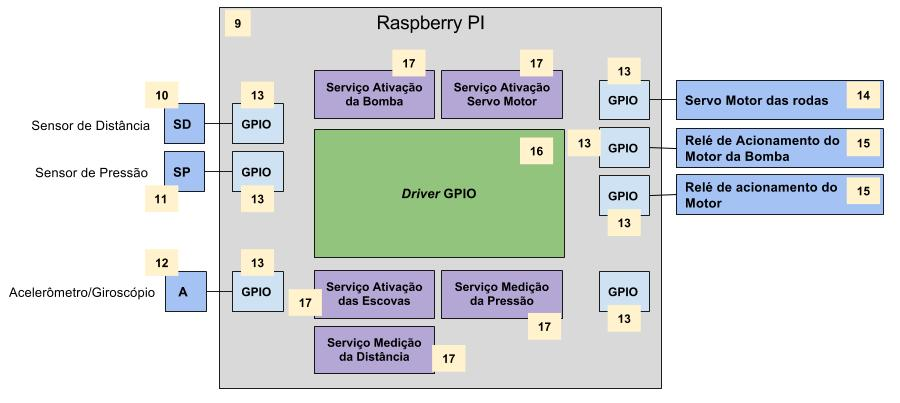
\includegraphics[width=0.9\textwidth]{figures/schema-interactive-eletro-soft.jpg}
  \caption{Esquemático da Interação entgre Eletrônica e Software}
  \label{fig:schema-interactive-electro-soft}
\end{figure}
\FloatBarrier
\par
A figura demonstra a interação dos componentes eletrônicos e o \textit{software}.
\par
Os periféricos fornecerão dados que, por sua vez, serão passados ao \textit{driver} por
meio de dispositivo de \textit{hardware} (GPIO).  O \textit{driver} será responsável por permitir
a comunicação entre o \textit{hardware} e o \textit{software} que, na figura, é representado pelos
serviços que deve fornecer ao sistema. Cada serviço tratará os dados de entrada
conforme a especificidade solicitada e, em seguida, retorna uma saída para um
atuador, por meio do \textit{driver}.
\par
\begin{description}
\item[\textit{Raspberry PI 2 B}:] Com o objetivo de desenvolver um robô é
necessário ter uma central de processamento de dados, a \textit{Raspberry pi} foi
escolhida pelo seu numero de portas GPIO aonde pode ser desenvolvido a solução
de sensores que existe para o problema, e também há a possibilidade de, caso
venham a aparecer a necessidade de mais sensores. A \textit{Raspberry pi} tem suporte a
sistema operacional, o que permite o uso de uma extensão maior de bibliotecas
como a biblioteca \textit{pthread}, também há a possibilidade do uso de varias linguagens
de programação.
\par
\begin{figure}[h]
  \centering
  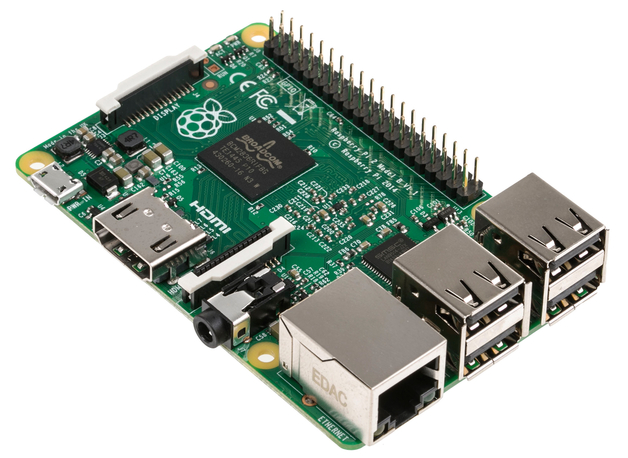
\includegraphics[width=0.8\textwidth]{figures/rpi2b.jpg}
  \caption{\textit{Raspberry Pi 2 B}}
  \label{fig:raspberry2b}
\end{figure}
\FloatBarrier

\item[GPIO:] \textit{Generic Ports Input Output} são saídas e entradas de tensão.
Elas servem para fazer a comunicação do processador com componentes externos,
sensores e atuadores e outros tipos de componentes eletrônicos. Algumas dessas
portas tem usos predefinidos pelo fabricante do \textit{hardware} como saídas de
alimentação genérica, e terras, outras dos pinos são de uso genérico. A
\textit{Raspberry pi} tem 40 GPIO, aonde dessas 17 são para uso genérico.
\par
\begin{figure}[h]
  \centering
  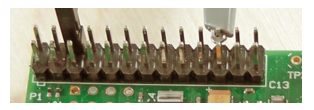
\includegraphics[width=0.6\textwidth]{figures/gpio.png}
  \caption{GPIO \textit{Raspberry Pi 2 B}}
  \label{fig:raspberry2b}
\end{figure}
\FloatBarrier

\item[Sensores de Distância:] serão utilizados sensores de distância com o
intuito de permitir ao robô a identificação do espaço entre o robô e qualquer
objeto à sua frente. Isso é importante para evitar colisões com as paredes da
piscina e obstáculos a alturas que o sensor possa detectar. O sensor específico
ainda não foi definido pois é necessário fazer teste com os propostos.

\item[Sensores de Pressão:] O sensor de pressão proposta funciona com o
princípios de materiais piezoelétricos, um liquido entra dentro da câmara
e proporciona uma pressão nas paredes da câmara, esse pressão gera uma
diferença de potencial no material. Com essa diferença de potencial é
possível, usando um conversor AD (Analógico/Digital), saber a pressão dentro
da câmara, e fora do robô.
\par
\begin{figure}[h]
  \centering
  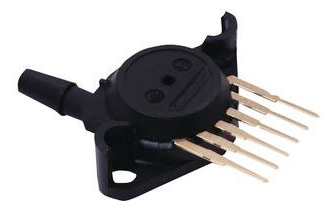
\includegraphics[width=0.6\textwidth]{figures/pressure-sensor.png}
  \caption{Sensor de pressão MPX4250GP}
  \label{fig:pressure-sensor}
\end{figure}
\FloatBarrier

\item[Acelerômetro/Giroscópio:] Está sendo cogitado usar um acelerômetro
para auxiliar o deslocamento em linha reta do robô e detectar choques com
obstáculos grandes, quando ocorre um choque com um obstaculo grande não
detectado pelo sensor de distancia a uma variação brusca na aceleração, com
isso podemos tratar o obstaculo ou abortar o funcionamento do robô.
\par
No mesmo módulo se encontra um giroscópio, ele mede rotações no robô, caso
seja identificado alguma rotação não pretendida pelo sistema podemos usar esse
dado para corrigir a trajetória do mesmo. O componente eletrônico que tem os
dois sensores se comunica através do protocolo I2C. Isso reduz o numero de
pinos necessários pare ler os dados do sensor.
\par
\begin{figure}[h]
  \centering
  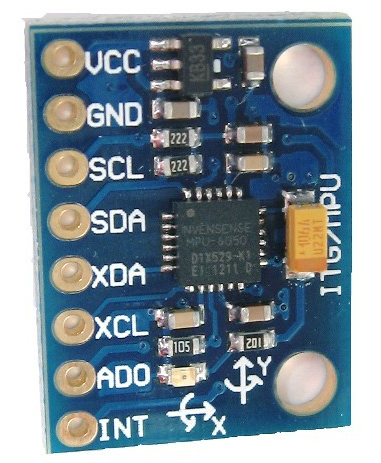
\includegraphics[width=0.5\textwidth]{figures/accelerometer.png}
  \caption{Acelerômetro/Giroscópio MPU-6050}
  \label{fig:accelerometer}
\end{figure}
\FloatBarrier

\item[Servo Motor:] Servos motores são utilizados para rotacionar um eixo até
uma posição desejada. Esses motores são normalmente motores de alto torque.
Dois servos (Micro Servo 9g SG90 TowerPro) serão utilizados para rotacionar
as rodas (5), o principal motivo de escolher esse modelo é ele ter torque
suficiente para mover as mesmas e ter baixo custo, E para mover a saída de água
(4) da bomba foi escolhido um servo motor (SM-S4306R) com maior liberdade de
rotação (360º) e uma maior torque.
\begin{figure}[h]
  \centering
	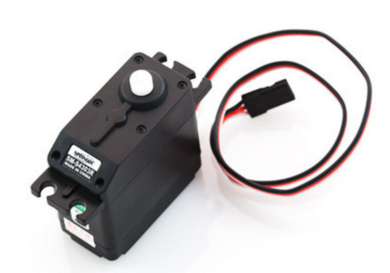
\includegraphics[height=5cm]{figures/servant-motor.png}
	\quad
	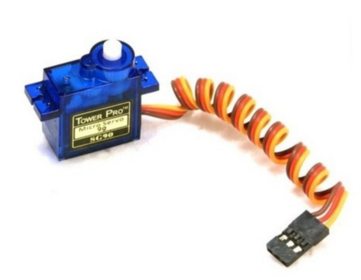
\includegraphics[height=5cm]{figures/micro-motor.png}
  \caption{Servo Motores.}
\end{figure}
\FloatBarrier

\item[Relé do Motor:] Os relés servem para fazer acionamento de circuitos
de alta tensão usando como chaves circuitos de baixa tensão, além disso os
 relés servem para isolar os circuitos de baixa tensão dos de alta tensão.
 
\item[\textit{Driver} GPIO:] O driver é um software que habilita a comunicação
entre o \textit{hardware} e o \textit{software}. A partir do driver é possível consumir os
dados advindos dos componentes de \textit{hardware}, fazer o devido tratamento e, se
necessário, enviar uma resposta ao\textit{hardware} \cite{windows2016}. Para o projeto foram
identificadas algumas bibliotecas, disponibilizadas pela comunidade que utiliza
o Raspberry. Essas bibliotecas fazem a interface entre o \textit{hardware} e o
\textit{middleware}, de forma que essas APIs fazem o papel do driver.

\item[\textit{Middleware} (Serviço):] é um \textit{software} que conecta outros componentes
de \textit{software}. Uma camada de infraestrutura que viabiliza o desenvolvimento de
aplicações voltadas ao negócio. Provê serviços que serão amplamente utilizados
pela aplicação de negócio \cite{oracle2016}. O middleware fornecerá serviços base para
o robô, como ativação dos motores, escova e uso dos sensores.
\end{description}

\subsection{Arquitetura de \textit{Software}}
A figura abaixo mostra a abstração da arquitetura do sistema associado ao projeto.
\par
\begin{figure}[h]
  \centering
  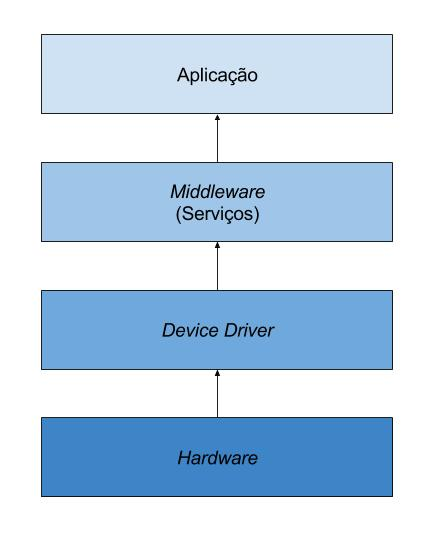
\includegraphics[width=0.4\textwidth]{figures/schema-arch.jpg}
  \caption{Arquitetura em Camadas do \textit{Software}.}
  \label{fig:schema-arch}
\end{figure}
\FloatBarrier

O sistema segue uma arquitetura em camadas. A partir do hardware os dados serão
capturados. O \textit{driver} fará a ponte de comunicação entre o \textit{hardware}
e o \textit{middleware}, permitindo que os dados possam ser trabalhados pela aplicação de
negócio. A aplicação de negócio utilizará os serviços disponíveis pelo \textit{middleware},
afim de tratar os dados recebidos e fornecer instruções ao robô. Uma visão
ampliada da arquitetura está disponível na figura abaixo.
\par
\begin{figure}[h]
  \centering
  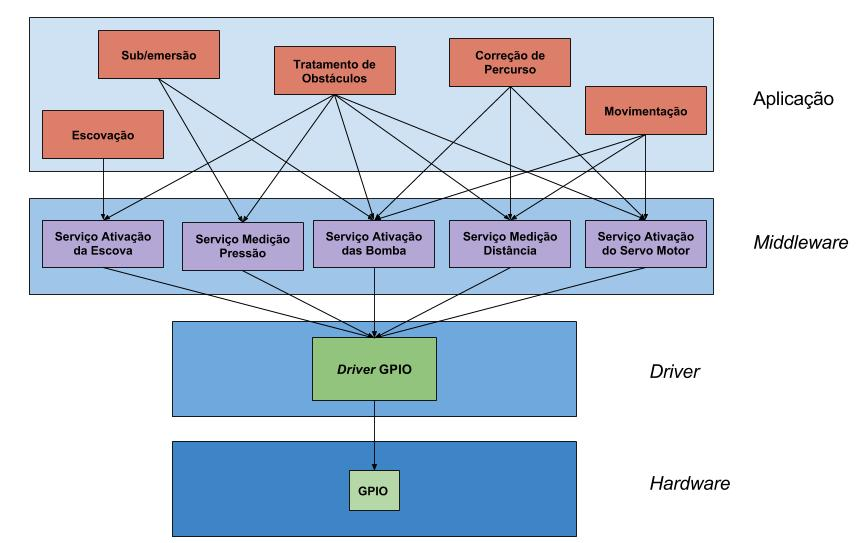
\includegraphics[width=0.9\textwidth]{figures/schema-layer-arch.jpg}
  \caption{Detalhamento das Camadas e Interação dos componentes}
  \label{fig:schema-layer-arch}
\end{figure}
\FloatBarrier